% article example for classicthesis.sty
\documentclass[10pt,a4paper]{article} % KOMA-Script article scrartcl
\usepackage{import}
\usepackage{xifthen}
\usepackage{pdfpages}
\usepackage{transparent}
\newcommand{\incfig}[1]{%
    \def\svgwidth{\columnwidth}
    \import{./figures/}{#1.pdf_tex}
}
\usepackage{lipsum}     %lorem ipsum text
\usepackage{titlesec}   %Section settings
\usepackage{titling}    %Title settings
\usepackage[margin=10em]{geometry}  %Adjusting margins
\usepackage{setspace}
\usepackage{listings}
\usepackage{amsmath}    %Display equations options
\usepackage{amssymb}    %More symbols
\usepackage{xcolor}     %Color settings
\usepackage{pagecolor}
\usepackage{mdframed}
\usepackage[spanish]{babel}
\usepackage[utf8]{inputenc}
\usepackage{longtable}
\usepackage{multicol}
\usepackage{graphicx}
\graphicspath{ {./Images/} }
\setlength{\columnsep}{1cm}

% ====| color de la pagina y del fondo |==== %



\begin{document}
    %========================{TITLE}====================%
    \title{{  Respuestas Parcial3  }}
    \author{{Rodrigo Castillo}}
    \date{\today}

    \maketitle


    %=======================NOTES GOES HERE===================%
    \section{Punto 2}
    \textbf{Algoritmo de Ford Fulkerson}

    \begin{figure}[h!]
        \centering
        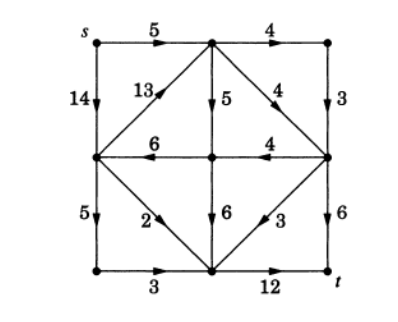
\includegraphics[width=0.4\linewidth]{grafodado.png}
        \caption{Grafo Dado}
        \label{fig}
    \end{figure}


    \section{Punto 3: Determine si el grafo dado es plano }
    \begin{figure}[h!]
        \centering
        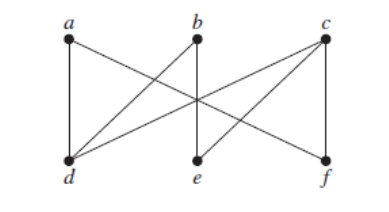
\includegraphics[width=0.4\linewidth]{plano.png}
        \caption{Es plano?}
        \label{fig}
    \end{figure}
    \textbf{Respuesta:El grafo si es plano puesto que no contiene a $K_5$ o a $K_{3,3}$}
    \\
    por lo que el grafo dibujado visto como plano es...
    \\
    \begin{figure}[ht]
        \centering
        \incfig{grafoplano}
        \caption{grafoplano}
        \label{fig:grafoplano}
    \end{figure}


    \section{Punto 4:Algoritmo del coloreado voraz}
    \textbf{el grafo de los estudiantes es de la siguiente manera:}
    \\
    \textbf{los vértices del grafo representan a los estudiantes}
    \\
    \textbf{las aristas del grafo representan las malas relaciones entre ellos}
    \\
    por lo que sabemos que el algoritmo de coloreado voraz sobre el grafo nos
    dará las rutas para el viaje, en el cuál cada color será una ruta diferente
    \begin{figure}[ht]
        \centering
        \incfig{grafoestudiantes}
        \caption{grafoestudiantes}
        \label{fig:grafoestudiantes}
    \end{figure}
    \textbf{por lo que son necesarias 3 rutas}


    \section{Punto 5 el tour del caballo}
    \textbf{a:modelo del problema}
    % ====|ACA EMPIEZA EL PUNTO 5-a|====
\begin{figure}[ht]
    \centering
    \incfig{problemacaballo}
    \caption{problemacaballo}
    \label{fig:problemacaballo}
\end{figure}



    % ====|ACA TERMINA EL PUNTO 5-a|==== %
    \textbf{b:problema en un tablero 3x3}
    \\
    para modelar este problema, haremos un grafo en el cuál cada vértice
    represente una casilla del ajedrez y cada arista represente los posibles
    movimientos de un caballo a las otras casillas
    \\
    \textbf{ejemplo:} sea la casilla $a-a$ como la casilla superior
    izquierda(en mi grafo el vértice $1,1$) sabemos que la casilla $a,a$ está
    conectada con la casilla $b,c$ y con la casilla $c,b$ , entonces , en el
    grafo , existirá una arista entre el vértice que representa la casilla
    $a,a$ y los vértices que representan las casillas $b,c$ y $c,b$
    \\
    \textbf{Problema del recorrido hamiltoniano}
    \\
    el problema de encontrar  un tour de caballo en un tablero de ajedrez es
    entonces análogo a encontrar un \textbf{recorrido hamiltoniano}  en el grafo definido
    previamente
    % ====|ACA EMPIEZA EL PUNTO 5-b|====

    \newpage
    representé este problema en el grafo $H$ , en el cuál sus vértices
    representan cada cuadro de un tablero de ajedrez y donde sus aristas
    representan los posibles movimientos de un caballo en ella .
    \\
    note que los movimientos de un caballo en un tablero de ajedrez , un
    grafo represeentan caminos de longitud 3 , además , en un tablero de
    ajedrez de 3x3 existe un vértice ($E$) cuya excentricidad es $2$ , por lo que no
    existe un camino de longitud 3 a ninguno de los otros vértices y por lo
    tanto es imposible llegar a el

    \begin{figure}[ht]
        \centering
        \incfig{tablero}
        \caption{tablero de ajedrez de 3x3}
        \label{fig:tablero}
    \end{figure}


    \begin{figure}[ht]
        \centering
        \incfig{grafo3por3}
        \caption{Grafo H (movimientos de caballo)}
        \label{fig:grafo3por3}
    \end{figure}



    % ====|ACA TERMINA EL PUNTO 5-b|==== %



















    %=======================NOTES ENDS HERE===================%

    % bib stuff
    \nocite{*}
    \addtocontents{toc}{{}}
    \addcontentsline{toc}{section}{\refname}
    \bibliographystyle{plain}
    \bibliography{../Bibliography}
\end{document}
